\documentclass[landscape,a5paper,11pt]{article}
\usepackage[utf8x]{inputenc} % utf8 encoding
\usepackage[T1]{fontenc} % use T1 fonts
\usepackage{amsmath} % nice math symbols
\usepackage{bm} % bold math
\usepackage{color} % change text color        

\usepackage{tikz}
\usetikzlibrary{decorations.pathmorphing} % for snake lines
\usetikzlibrary{matrix} % for block alignment
\usetikzlibrary{arrows} % for arrow heads
\usetikzlibrary{calc} % for manimulation of coordinates

% TikZ styles for drawing
\tikzstyle{block} = [draw,rectangle,thick,minimum height=2em,minimum width=2em]
\tikzstyle{sum} = [draw,circle,inner sep=0mm,minimum size=2mm]
\tikzstyle{connector} = [->,thick]
\tikzstyle{line} = [thick]
\tikzstyle{branch} = [circle,inner sep=0pt,minimum size=1mm,fill=black,draw=black]
\tikzstyle{guide} = []
\tikzstyle{snakeline} = [connector, decorate, decoration={pre length=0.2cm,
                         post length=0.2cm, snake, amplitude=.4mm,
                         segment length=2mm},thick, magenta, ->]

\renewcommand{\vec}[1]{\ensuremath{\boldsymbol{#1}}} % bold vectors
\def \myneq {\skew{-2}\not =} % \neq alone skews the dash

\begin{document}

  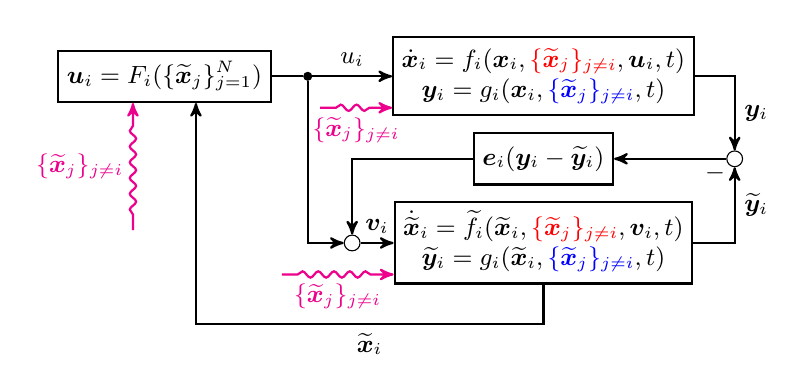
\begin{tikzpicture}[scale=1, auto, >=stealth']
    \small
    % node placement with matrix library: 5x4 array
    \matrix[ampersand replacement=\&, row sep=0.2cm, column sep=0.4cm] {
      %
      \node[block] (F1) {$\vec{u}_i = F_i(\{\widetilde{\vec{x}}_j\}_{j=1}^N)$}; \&
      \node[branch] (u1) {}; \&
      \&
      \node[block] (f1) {$\begin{matrix}
            \dot{\vec{x}}_i =
              f_i(\vec{x}_i,
                  \textcolor{red}{\{\widetilde{\vec{x}}_j\}_{j \myneq i}},
                  \vec{u}_i,
                  t)\\
            \vec{y}_i =
              g_i(\vec{x}_i,
                  \textcolor{blue}{\{\widetilde{\vec{x}}_j\}_{j \myneq i}},
                  t)
          \end{matrix}$}; \& \\

      \&
      \&
      \&
      \node[block] (L1) {$\vec{e}_i(\vec{y}_i - \widetilde{\vec{y}}_i)$};\&
      \node [sum] (e1) {}; \\

      \&
      \&
      \node[sum] (v1) {}; \&
      \node[block] (o1) {$\begin{matrix}
            \dot{\widetilde{\vec{x}}}_i =
              \widetilde{f}_i(\widetilde{\vec{x}}_i,
                              \textcolor{red}{\{\widetilde{\vec{x}}_j\}_{j \myneq i}},
                              \vec{v}_i, t)\\
              \widetilde{\vec{y}}_i =
                g_i(\widetilde{\vec{x}}_i,
                    \textcolor{blue}{\{\widetilde{\vec{x}}_j\}_{j \myneq i}},
                    t)
          \end{matrix}$};
      \&
      \\
      \node[guide] (i1) {}; \& \& \& \& \\
    };

    % now link the nodes
    \draw [line] (F1) -- (u1);
    \draw [connector] (u1) -- node {$u_i$} (f1);
    \draw [connector] (f1) -| node[near end] {$\vec{y}_i$} (e1);
    \draw [connector] (e1) -- (L1);
    \draw [connector] (L1) -| (v1);
    \draw [connector] (v1) -- node {$\vec{v}_i$} (o1);
    \draw [connector] (u1) |- (v1);
    \draw [connector] (o1) -| node[pos=0.96] {$-$} node [near end, swap]
                      {$\widetilde{\vec{y}}_i$} (e1);
    \draw [connector] (o1.south) -- ++(0,-.5cm) -| node [near start]
                      {$\widetilde{\vec{x}}_i$} ($(F1.south) + (0.4cm, 0em)$);
    
    % draw the snake lines with offset (using the calc library)
    \draw [snakeline] ($(i1) - (0.4cm, -1cm)$) -- node
      {$\{\widetilde{\vec{x}}_j\}_{j \myneq i}$} ($(F1.south) - (0.4cm, 0em)$);

    \draw [snakeline, swap] ($(v1.east) - (1.0cm, 0.4cm)$) -- node
      {$\{\widetilde{\vec{x}}_j\}_{j \myneq i}$} ($(o1.west) - (0cm, 0.4cm)$);
    
    \draw [snakeline, swap] ($(u1.east) + (0.1cm, -0.4cm)$) -- node
      {$\{\widetilde{\vec{x}}_j\}_{j \myneq i}$} ($(f1.west) - (0cm, 0.4cm)$);

  \end{tikzpicture}

\end{document}
